\documentclass[11pt,a4paper]{article}

\usepackage[margin=0.5in, top=3cm, bottom=2cm]{geometry}
\usepackage[spanish, activeacute]{babel}
\usepackage[utf8]{inputenc}
\usepackage{amsthm}
\usepackage{amsmath}
\usepackage{amsfonts}
\usepackage{amssymb}
\usepackage{graphicx} %Para incluir el logo de la UBA
\usepackage{caratula} %Para armar el cuadro de integrantes
\usepackage{todonotes}
\usepackage{float}
\usepackage[lined,ruled,linesnumbered]{algorithm2e}
\usepackage{hyperref}
\usepackage{xcolor}
\usepackage[final]{pdfpages}
\providecommand{\DontPrintSemicolon}{\dontprintsemicolon}

\graphicspath{{imagenes/}}

\newcommand\comentario[2]{\textbf{{[#1: \textcolor{red}{#2}}}]}
\renewcommand\comentario[2]{}

\setcounter{secnumdepth}{5}

\begin{document}

\integrante{Maurizio, Miguel Sebasti\'{a}n}{635/11}{miguelmaurizio.92@gmail.com}
\integrante{Prillo, Sebasti\'{a}n}{616/11}{sebastianprillo@gmail.com}
\integrante{Tagliavini Ponce, Guido}{783/11}{guido.tag@gmail.com}

\def\Materia{Bases de Datos}
\def\Titulo{Trabajo Pr\'{a}ctico 1}
\def\Fecha{9 de agosto de 2015}

%----- CARATULA -----%

\thispagestyle{empty}

\begin{center}
	
\includegraphics[scale = 0.25]{imagenes/logo_uba.jpg}
\end{center}

\begin{center}
	{\textbf{\large UNIVERSIDAD DE BUENOS AIRES}}\\[1.5em]
	{\textbf{\large Departamento de Computaci\'{o}n}}\\[1.5em]
    {\textbf{\large Facultad de Ciencias Exactas y Naturales}}\\
    \vspace{35mm}
    {\LARGE\textbf{\Materia}}\\[1em]    
    \vspace{15mm}
    {\Large \textbf{\Titulo}}\\[1em]
    \vspace{15mm}
    {\textbf{\Large \Fecha}}\\
    \vspace{15mm}
    \textbf{\tablaints}
\end{center}

\newpage
\thispagestyle{empty}
\tableofcontents

\parskip=5pt
\setlength{\parindent}{0pt}

\newpage
\setcounter{page}{1}
\pagenumbering{arabic}
\pagestyle{plain}

\section{Introducci'on}
\section{Diagrama Entidad Relaci'on}

A partir de los requerimientos recabados, elaboramos un diagrama de entidad-relaci'on, que presentamos a continuaci'on.

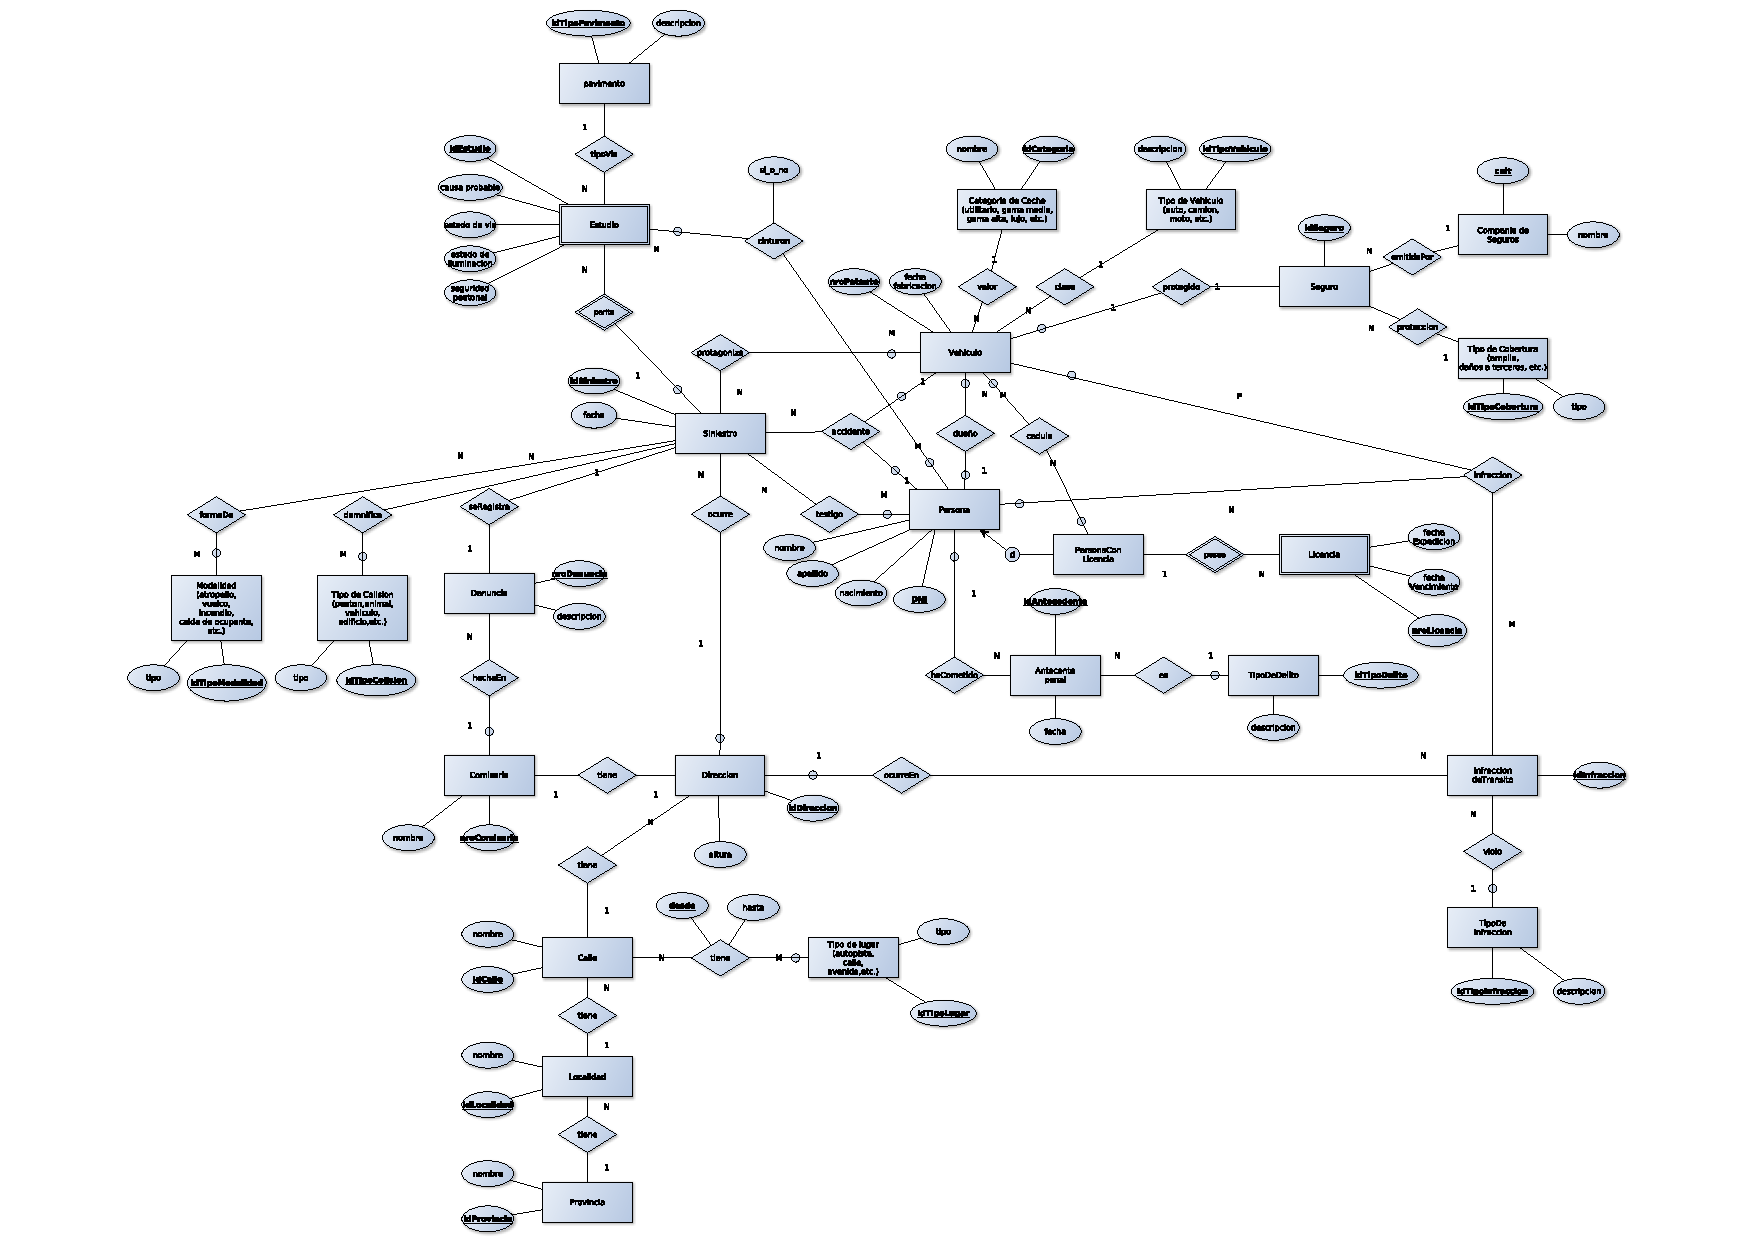
\includepdf[pages=-,angle=90]{imagenes/DER.pdf}

\subsection{Restricciones en lenguaje natural}

Las restricciones que el DER no puede capturar son las siguientes:

\begin{enumerate}
\item Las personas relacionadas con un estudio, deben estar involucradas en el siniestro correspondiente a ese estudio.

\item Si un veh'iculo sin conductor forma parte de un siniestro (es decir, est'a relacionado con un siniestro v'ia la relaci'on binaria \textit{protagoniza}), entones no era conducido por nadie en ese siniestro (es decir, no aparece en la relaci'on ternaria \textit{accidente} con ese siniestro).

\item Las personas que aparecen relacionadas con el estudio en la relacion \textit{cinturon}, deben ser personas que participaron del siniestro correspondiente al estudio, conduciendo uno de los vehiculos de ese siniestro.

\item Cada persona aparece a lo sumo una vez por siniestro. En otras palabras, un siniestro no puede estar relacionado dos veces con la misma persona v'ia la ternaria \textit{accidente}.

\item Cada vehiculo aparece a lo sumo una vez por siniestro. En otras palabras, un siniestro no puede estar relacionado dos veces con el mismo veh'iculo v'ia la ternaria \textit{accidente}.

\item No hay solapamiento entre los rangos de alturas de las calles. Por ejemplo, no puede ser que Monroe del 0 al 3000 sea calle y del 2500 al 4000 sea avenida.

\end{enumerate}

\section{Modelo Relacional}

A partir del DER, derivamos el siguiente modelo relacional. Lo presentamos directamente en sintaxis SQL.

Algunas de las relaciones N-M del DER ten'ian nombres poco ilustrativos al ser sacados de contexto. Por ejemplo, la relaci'on binaria entre \textit{Siniestro} y \textit{Tipo de Colisi'on} fue llamada \textit{damnifica}, nombre que no tiene mucho sentido aisladamente. Esto representaba un problema, dado que en, el MR, esas relaciones pasan a ser tablas. En estos casos, decidimos transformar el nombre de estas relaciones, usando los nombres de las entidades relacionadas, del siguiente modo. Una relaci'on de nombre \textit{R} entre dos entidades de nombres \textit{X} e \textit{Y}, se pasa a llamar \textit{X\_R\_Y}. Por ejemplo, en el caso de la relaci'on \textit{damnifica}, el nombre de la tabla asociada pas'o a ser \textit{siniestro\_damnifica\_tipo\_de\_colision}. En algunos casos, los nombres eran suficientemente autoexplicativos, y no fue necesario hacer este cambio. Incluimos, arriba de cada sentencia \texttt{CREATE TABLE}, la entidad o relaci'on correspondiente a la tabla creada.

\begin{verbatim}
-- entidad Provincia
CREATE TABLE provincia (
 idProvincia INTEGER NOT NULL,
 nombre VARCHAR(255) NOT NULL,
 PRIMARY KEY(idProvincia)
);

-- entidad Localidad
CREATE TABLE localidad (
 idLocalidad INTEGER NOT NULL,
 nombre VARCHAR(255) DEFAULT NULL,
 idProvincia INTEGER NOT NULL,
 PRIMARY KEY(idLocalidad,idProvincia),
 FOREIGN KEY(idProvincia) REFERENCES provincia(idProvincia)
);

-- entidad Calle
CREATE TABLE calle (
 idCalle INTEGER NOT NULL,
 nombre VARCHAR(255) DEFAULT NULL,
 idLocalidad INTEGER NOT NULL,
 idProvincia INTEGER NOT NULL,
 PRIMARY KEY(idCalle,idLocalidad,idProvincia),
 FOREIGN KEY(idLocalidad,idProvincia) REFERENCES localidad(idLocalidad,idProvincia)
);

-- entidad Direccion
CREATE TABLE direccion (
 altura INTEGER NOT NULL,
 idCalle INTEGER NOT NULL,
 idLocalidad INTEGER NOT NULL,
 idProvincia INTEGER NOT NULL,
 PRIMARY KEY(altura,idCalle,idLocalidad,idProvincia),
 FOREIGN KEY(idCalle,idLocalidad,idProvincia) REFERENCES calle(idCalle,idLocalidad,idProvincia)
);

-- entidad Tipo de Lugar
CREATE TABLE tipo_de_lugar (
 idTipoLugar INTEGER NOT NULL,
 tipo VARCHAR(255) DEFAULT NULL,
 PRIMARY KEY(idTipoLugar)
);

-- relacion tiene, entre Calle y Tipo de Lugar
CREATE TABLE calle_tiene_tipo_de_lugar (
 idCalle INTEGER NOT NULL,
 idLocalidad INTEGER NOT NULL,
 idProvincia INTEGER NOT NULL,
 idTipoLugar INTEGER NOT NULL,
 desde INTEGER NOT NULL,
 hasta INTEGER NOT NULL,
 PRIMARY KEY(idCalle, idLocalidad, idProvincia, idTipoLugar, desde),
 FOREIGN KEY(idCalle, idLocalidad, idProvincia) REFERENCES calle(idCalle,idLocalidad,idProvincia),
 FOREIGN KEY(idTipoLugar) REFERENCES tipo_de_lugar(idTipoLugar)
);

-- entidad Comisaria
CREATE TABLE comisaria (
 nroComisaria INTEGER NOT NULL,
 nombre VARCHAR(255) DEFAULT NULL,
 altura INTEGER NOT NULL,
 idCalle INTEGER NOT NULL,
 idLocalidad INTEGER NOT NULL,
 idProvincia INTEGER NOT NULL,
 PRIMARY KEY(nroComisaria),
 FOREIGN KEY(altura,idCalle,idLocalidad,idProvincia) REFERENCES direccion(idDireccion,idCalle,idLocalidad,idProvincia)
);

-- entidad Denuncia
CREATE TABLE denuncia (
 nroDenuncia INTEGER NOT NULL,
 descripcion VARCHAR(255) DEFAULT NULL,
 nroComisaria INTEGER NOT NULL,
 PRIMARY KEY(nroDenuncia),
 FOREIGN KEY(nroComisaria) REFERENCES comisaria(nroComisaria)
);

-- entidad Tipo de Colision
CREATE TABLE tipo_de_colision (
 idTipoColision INTEGER NOT NULL,
 tipo VARCHAR(255) DEFAULT NULL,
 PRIMARY KEY(idTipoColision)
);

-- entidad Modalidad
CREATE TABLE modalidad (
 idTipoModalidad INTEGER NOT NULL,
 tipo VARCHAR(255) DEFAULT NULL,
 PRIMARY KEY(idTipoModalidad)
);

-- entidad Siniestro
CREATE TABLE siniestro (
 idSiniestro INTEGER NOT NULL,
 fecha DATETIME DEFAULT NULL,
 nroDenuncia INTEGER NOT NULL,
 altura INTEGER NOT NULL,
 idCalle INTEGER NOT NULL,
 idLocalidad INTEGER NOT NULL,
 idProvincia INTEGER NOT NULL,
 PRIMARY KEY(idSiniestro),
 FOREIGN KEY(nroDenuncia) REFERENCES denuncia(nroDenuncia),
 FOREIGN KEY(altura,idCalle,idLocalidad,idProvincia) REFERENCES direccion(altura,idCalle,idLocalidad,idProvincia)
);

-- relacion damnifica, entre Siniestro y Tipo de Colision
CREATE TABLE siniestro_damnifica_tipo_de_colision (
 idSiniestro INTEGER NOT NULL,
 idTipoColision INTEGER NOT NULL,
 PRIMARY KEY(idSiniestro, idTipoColision),
 FOREIGN KEY(idSiniestro) REFERENCES siniestro(idSiniestro),
 FOREIGN KEY(idTipoColision) REFERENCES tipo_de_colision(idTipoColision)
);

-- relacion formaDe, entre Siniestro y Modalidad
CREATE TABLE siniestro_forma_de_modalidad (
 idSiniestro INTEGER NOT NULL,
 idTipoModalidad INTEGER NOT NULL,
 PRIMARY KEY(idSiniestro, idTipoModalidad),
 FOREIGN KEY(idSiniestro) REFERENCES siniestro(idSiniestro),
 FOREIGN KEY(idTipoModalidad) REFERENCES modalidad(idTipoModalidad)
);

-- entidad Tipo de Pavimento
CREATE TABLE tipo_de_pavimento (
 idTipoPavimento INTEGER NOT NULL,
 descripcion VARCHAR(255) DEFAULT NULL,
 PRIMARY KEY(idTipoPavimento)
);

-- entidad Estudio
CREATE TABLE estudio (
 idEstudio INTEGER NOT NULL,
 causaProbable VARCHAR(255) DEFAULT NULL,
 estadoVia VARCHAR(255) DEFAULT NULL,
 estadoIluminacion VARCHAR(255) DEFAULT NULL,
 seguridadPeatonal BOOLEAN DEFAULT NULL,
 idTipoPavimento INTEGER NOT NULL,
 idSiniestro INTEGER NOT NULL,
 PRIMARY KEY (idEstudio, idSiniestro),
 FOREIGN KEY(idTipoPavimento) REFERENCES tipo_de_pavimento(idTipoPavimento),
 FOREIGN KEY(idSiniestro) REFERENCES siniestro(idSiniestro)
);

-- entidad Persona
CREATE TABLE persona (
 dni INTEGER NOT NULL,
 nombre VARCHAR(255) NOT NULL,
 apellido VARCHAR(255) NOT NULL,
 nacimiento DATE NOT NULL,
 PRIMARY KEY(dni)
);

-- relacion testigo, entre Siniestro y Persona
CREATE TABLE siniestro_testigo_persona (
 idSiniestro INTEGER NOT NULL,
 dni INTEGER NOT NULL,
 PRIMARY KEY(idSiniestro, dni),
 FOREIGN KEY(idSiniestro) REFERENCES siniestro(idSiniestro),
 FOREIGN KEY(dni) REFERENCES persona(dni)
);

-- relacion cinturon, entre Estudio y Persona
CREATE TABLE estudio_cinturon_persona (
 idEstudio INTEGER NOT NULL,
 dni INTEGER NOT NULL,
 si_o_no BOOLEAN NOT NULL,
 PRIMARY KEY(idEstudio, dni),
 FOREIGN KEY(idEstudio) REFERENCES estudio(idEstudio),
 FOREIGN KEY(dni) REFERENCES persona(dni)
);

-- entidad Tipo de Delito
CREATE TABLE tipo_de_delito (
 idTipoDelito INTEGER NOT NULL,
 descripcion VARCHAR(255) DEFAULT NULL,
 PRIMARY KEY(idTipoDelito)
);

-- entidad Antecedente Penal
CREATE TABLE antecedente_penal (
 idAntecedente INTEGER NOT NULL,
 fecha Date NOT NULL,
 dni INTEGER NOT NULL,
 idTipoDelito INTEGER NOT NULL,
 FOREIGN KEY(dni) REFERENCES persona(dni),
 FOREIGN KEY(idTipoDelito) REFERENCES tipo_de_delito(idTipoDelito),
 PRIMARY KEY(idAntecedente)
);

-- entidad Tipo de Infraccion
CREATE TABLE tipo_de_infraccion (
 idTipoInfraccion INTEGER NOT NULL,
 descripcion VARCHAR(255) DEFAULT NULL,
 PRIMARY KEY(idTipoInfraccion)
);

-- entidad Infraccion de Transito
CREATE TABLE infraccion_de_transito (
 idInfraccion INTEGER NOT NULL,
 altura INTEGER NOT NULL,
 idCalle INTEGER NOT NULL,
 idLocalidad INTEGER NOT NULL,
 idProvincia INTEGER NOT NULL,
 idTipoInfraccion INTEGER NOT NULL,
 FOREIGN KEY(altura,idCalle,idLocalidad,idProvincia) REFERENCES direccion(idDireccion,idCalle,idLocalidad,idProvincia),
 FOREIGN KEY(idTipoInfraccion) REFERENCES tipo_infraccion(idTipoInfraccion),
 PRIMARY KEY(idInfraccion)
);

-- entidad Persona con Licencia
CREATE TABLE persona_con_licencia (
 dni INTEGER NOT NULL,
 FOREIGN KEY(dni) REFERENCES persona(dni),
 PRIMARY KEY(dni)
);

-- entidad Licencia
CREATE TABLE licencia (
 nroLicencia INTEGER NOT NULL,
 dni INTEGER NOT NULL,
 expedicion DATE NOT NULL,
 expiracion DATE NOT NULL,
 FOREIGN KEY(dni) REFERENCES persona_con_licencia(dni),
 PRIMARY KEY (nroLicencia, dni)
);

-- entidad Compania de Seguros
CREATE TABLE compania_de_seguro (
 cuit INTEGER NOT NULL,
 nombre VARCHAR(255) NOT NULL,
 PRIMARY KEY(cuit)
);

-- entidad Tipo de Cobertura
CREATE TABLE tipo_de_cobertura (
 idTipoCobertura INTEGER NOT NULL,
 descripcion VARCHAR(255) NOT NULL,
 PRIMARY KEY(idTipoCobertura)
);

-- entidad Tipo de Vehiculo
CREATE TABLE tipo_de_vehiculo (
 idTipoVehiculo INTEGER NOT NULL,
 descripcion VARCHAR(255) NOT NULL,
 PRIMARY KEY(idTipoVehiculo)
);

-- entidad Categoria de Coche
CREATE TABLE categoria_de_vehiculo (
 idCategoria INTEGER NOT NULL,
 descripcion VARCHAR(255) NOT NULL,
 PRIMARY KEY(idCategoria)
);

-- entidad Vehiculo
CREATE TABLE vehiculo (
 nroPatente CHARACTER(6) NOT NULL,
 fechaFabricacion DATE NOT NULL,
 idCategoria INTEGER NOT NULL,
 idTipoVehiculo INTEGER NOT NULL,
 dni INTEGER NOT NULL,
 FOREIGN KEY(idCategoria) REFERENCES categoria_de_vehiculo(idCategoria),
 FOREIGN KEY(idTipoVehiculo) REFERENCES tipo_de_vehiculo(idTipoVehiculo),
 FOREIGN KEY(dni) REFERENCES persona(dni),
 PRIMARY KEY(nroPatente)
);

-- entidad Seguro
CREATE TABLE seguro (
 idSeguro INTEGER NOT NULL,
 cuit INTEGER NOT NULL,
 idTipoCobertura INTEGER NOT NULL,
 nroPatente INTEGER NOT NULL,
 FOREIGN KEY(cuit) REFERENCES compania_de_seguro(cuit),
 FOREIGN KEY(idTipoCobertura) REFERENCES cobertura(idTipoCobertura),
 FOREIGN KEY(nroPatente) REFERENCES vehiculo(nroPatente),
 PRIMARY KEY(idSeguro)
);

-- relacion cedula, entre Vehiculo y Persona con Licencia
CREATE TABLE cedula (
 nroPatente CHARACTER(6) NOT NULL,
 dni INTEGER NOT NULL,
 FOREIGN KEY(nroPatente) REFERENCES vehiculo(nroPatente),
 FOREIGN KEY(dni) REFERENCES persona_con_licencia(dni),
 PRIMARY KEY(nroPatente, dni)
);

-- relacion protagoniza, entre Siniesto y Vehiculo
CREATE TABLE siniestro_protagoniza_vehiculo (
 nroPatente CHARACTER(6) NOT NULL,
 idSiniestro INTEGER NOT NULL,
 FOREIGN KEY(nroPatente) REFERENCES vehiculo(nroPatente),
 FOREIGN KEY(idSiniestro) REFERENCES siniestro(idSiniestro),
 PRIMARY KEY(nroPatente, idSiniestro)
);

-- relacion accidente, entre Siniestro, Vehiculo y Persona
CREATE TABLE siniestro_vehiculo_persona (
 nroPatente CHARACTER(6) NOT NULL,
 idSiniestro INTEGER NOT NULL,
 dni INTEGER NOT NULL,
 culpable BOOLEAN NOT NULL,
 FOREIGN KEY(nroPatente) REFERENCES vehiculo(nroPatente),
 FOREIGN KEY(idSiniestro) REFERENCES siniestro(idSiniestro),
 FOREIGN KEY(dni) REFERENCES persona(dni), 
 PRIMARY KEY(nroPatente, idSiniestro)
);

-- relacion infraccion, entre Persona, Vehiculo e Infraccion de Transito
CREATE TABLE persona_en_vehiculo_comete_infraccion (
 nroPatente CHARACTER(6) NOT NULL,
 dni INTEGER NOT NULL,
 idInfraccion INTEGER NOT NULL,
 FOREIGN KEY(nroPatente) REFERENCES vehiculo(nroPatente),
 FOREIGN KEY(dni) REFERENCES persona(dni), 
 FOREIGN KEY(idInfraccion) REFERENCES infraccion_de_transito(idInfraccion), 
 PRIMARY KEY(nroPatente, dni, idInfraccion)
);
\end{verbatim}

%\section{Supuestos Asumidos}



\section{Implementaci'on}



%\section{Consultas}



%\section{Conclusi'on}

En este trabajo hemos estudiado dos modelos de bases de datos no relacionales.

Por un lado, hemos visto, en profundidad, c'omo realizar un modelado de una \textit{document oriented}, responder consultas sobre la base de datos, realizar consultas MapReduce, y aplicar t'ecnicas de sharding para que los accesos a la base de datos en un hipot'etico escenario de clustering, sea eficiente. Se pudo ver que este el modelado en esta clase de bases de datos es sencillo, y permite que las consultas sean m'as sencillas que en SQL tradicional, puesto que este dise\~no se orienta espec'ificamente a responder las consultas de nuestro inter'es. La capacidad de realizar consultas MapReduce y de utilizar sharding ponen en evidencia lo preparado de esta clase de base de datos para un escenario de c'omputo distribu'ido, en el cual los datos se distribuyen sobre m'as de una computadora. Bajo ciertas hip'otesis de uniformidad sobre la informaci'on ingresada en la base de datos, mostramos que el sharding permite balancear la carga de datos sobre todos los shards, lo cual, en el mundo real, tiene un impacto no s'olo en la optimizaci'on de los recursos de hardware (ning'un nodo requiere demasiado disco), sino tambi'en desde el punto de vista del tiempo de respuesta de las queries (el ancho de banda necesario para mantener un delay aceptable es bajo, pues no hay nodos que sean cuellos de botella).
Adem'as, en muchos casos donde se trabaja con cantidades enormes de datos, SQL es imposible de utilizar. La gran ventaja de las bases de NOSQL es que permite que escalen en forma horizontal, ademas de vertical. Es decir, hablando en forma simplificada, para procesar un mayor flujo en SQL tradicional necesitamos una $mejor$ computadora, en cambio en NOSQL podemos utilizar una $mayor cantidad$ de computadoras.
Por otro lado, estudiamos superficialmente el modelo \textit{column oriented}. Como se vi'o, este modelo provee prestaciones similares, al permitir tanto consultas MapReduce como sharding. La disyuntiva en la elecci'on entre document oriented y column oriented depender'a fuertemente del contexto en el que estemos trabajando. De hecho, incluso dentro de una misma familia, dada la gran cantidad de oferta de bases de datos NOSQL, existen diferentes implementaciones, con ventajas y desventajas que el desarrollador deber'a evaluar a la hora de su elecci'on.


\bibliographystyle{plain}
\bibliography{main}

\end{document}
